\documentclass[a4paper,12pt]{article}

%%% Работа с русским языком
\usepackage{cmap}					% поиск в PDF
\usepackage{mathtext} 				% русские буквы в формулах
\usepackage[T2A]{fontenc}			% кодировка
\usepackage[utf8]{inputenc}			% кодировка исходного текста
\usepackage[english,russian]{babel}	% локализация и переносы
\usepackage{xcolor}
\usepackage{hyperref}
 % Цвета для гиперссылок
\definecolor{linkcolor}{HTML}{799B03} % цвет ссылок
\definecolor{urlcolor}{HTML}{799B03} % цвет гиперссылок

\hypersetup{pdfstartview=FitH,  linkcolor=linkcolor,urlcolor=urlcolor, colorlinks=true}

%%% Дополнительная работа с математикой
\usepackage{amsfonts,amssymb,amsthm,mathtools} % AMS
\usepackage{amsmath}
\usepackage{icomma} % "Умная" запятая: $0,2$ --- число, $0, 2$ --- перечисление

%% Номера формул
%\mathtoolsset{showonlyrefs=true} % Показывать номера только у тех формул, на которые есть \eqref{} в тексте.

%% Шрифты
\usepackage{euscript}	 % Шрифт Евклид
\usepackage{mathrsfs} % Красивый матшрифт

%% Свои команды
\DeclareMathOperator{\sgn}{\mathop{sgn}}

%% Перенос знаков в формулах (по Львовскому)
\newcommand*{\hm}[1]{#1\nobreak\discretionary{}
{\hbox{$\mathsurround=0pt #1$}}{}}
% графика
\usepackage{graphicx}
\graphicspath{{pictures/}}

\usepackage[left=25mm, top=30mm, right=25mm, bottom=30mm, nohead, nofoot]{geometry}

\DeclareGraphicsExtensions{.pdf,.png,.jpg}
\author{Бурмашев Григорий, БПМИ-208}
\title{Язык SQL, дз -- 11}
\date{\today}
\begin{document}
\maketitle
\clearpage
Для работы с полнотекстовым поиском использовал пример из презентации:
\begin{center}

\includegraphics[scale=0.4]{1.png}
\end{center}
\begin{center}
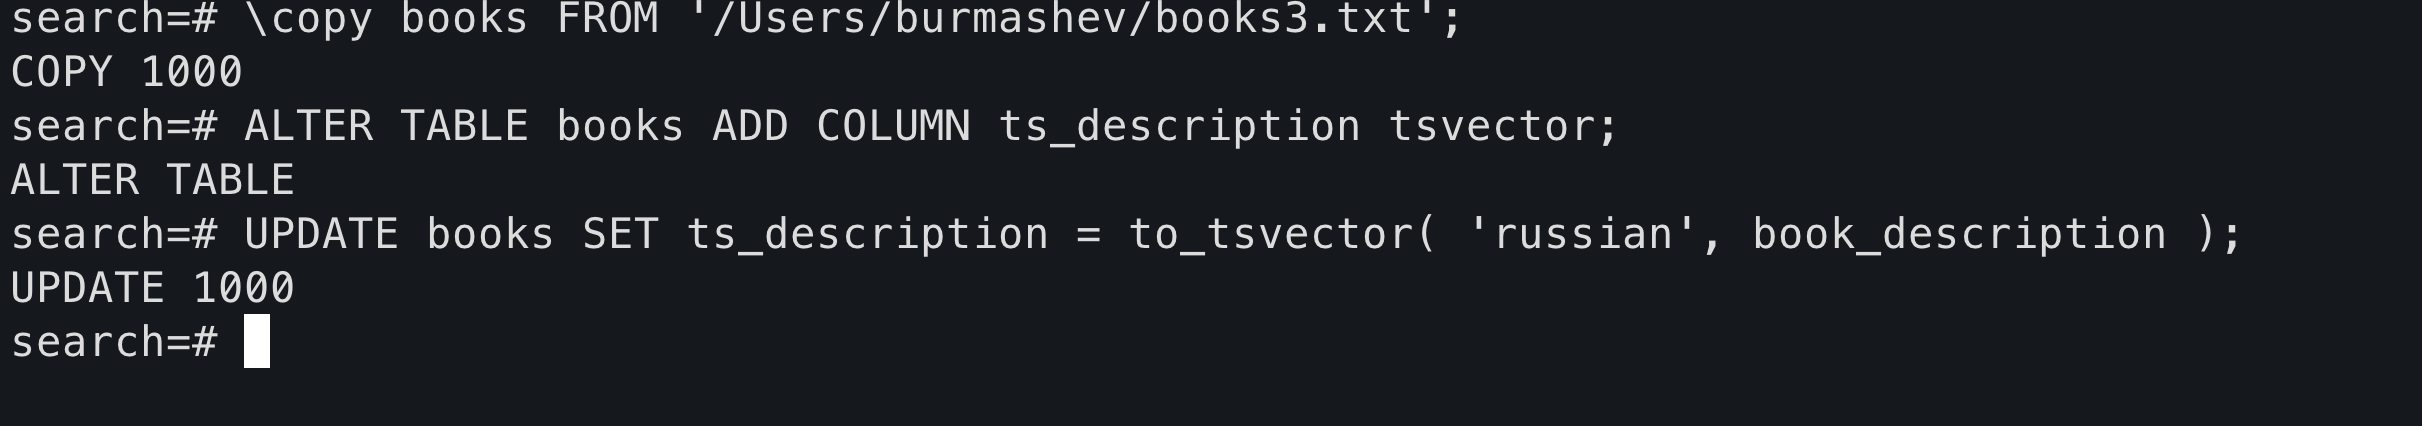
\includegraphics[scale=0.4]{2.png}
\end{center}
Пример использования полнотекстового поиска:
\\\\
Книги про программирование, изданные в Москве:
\begin{center}
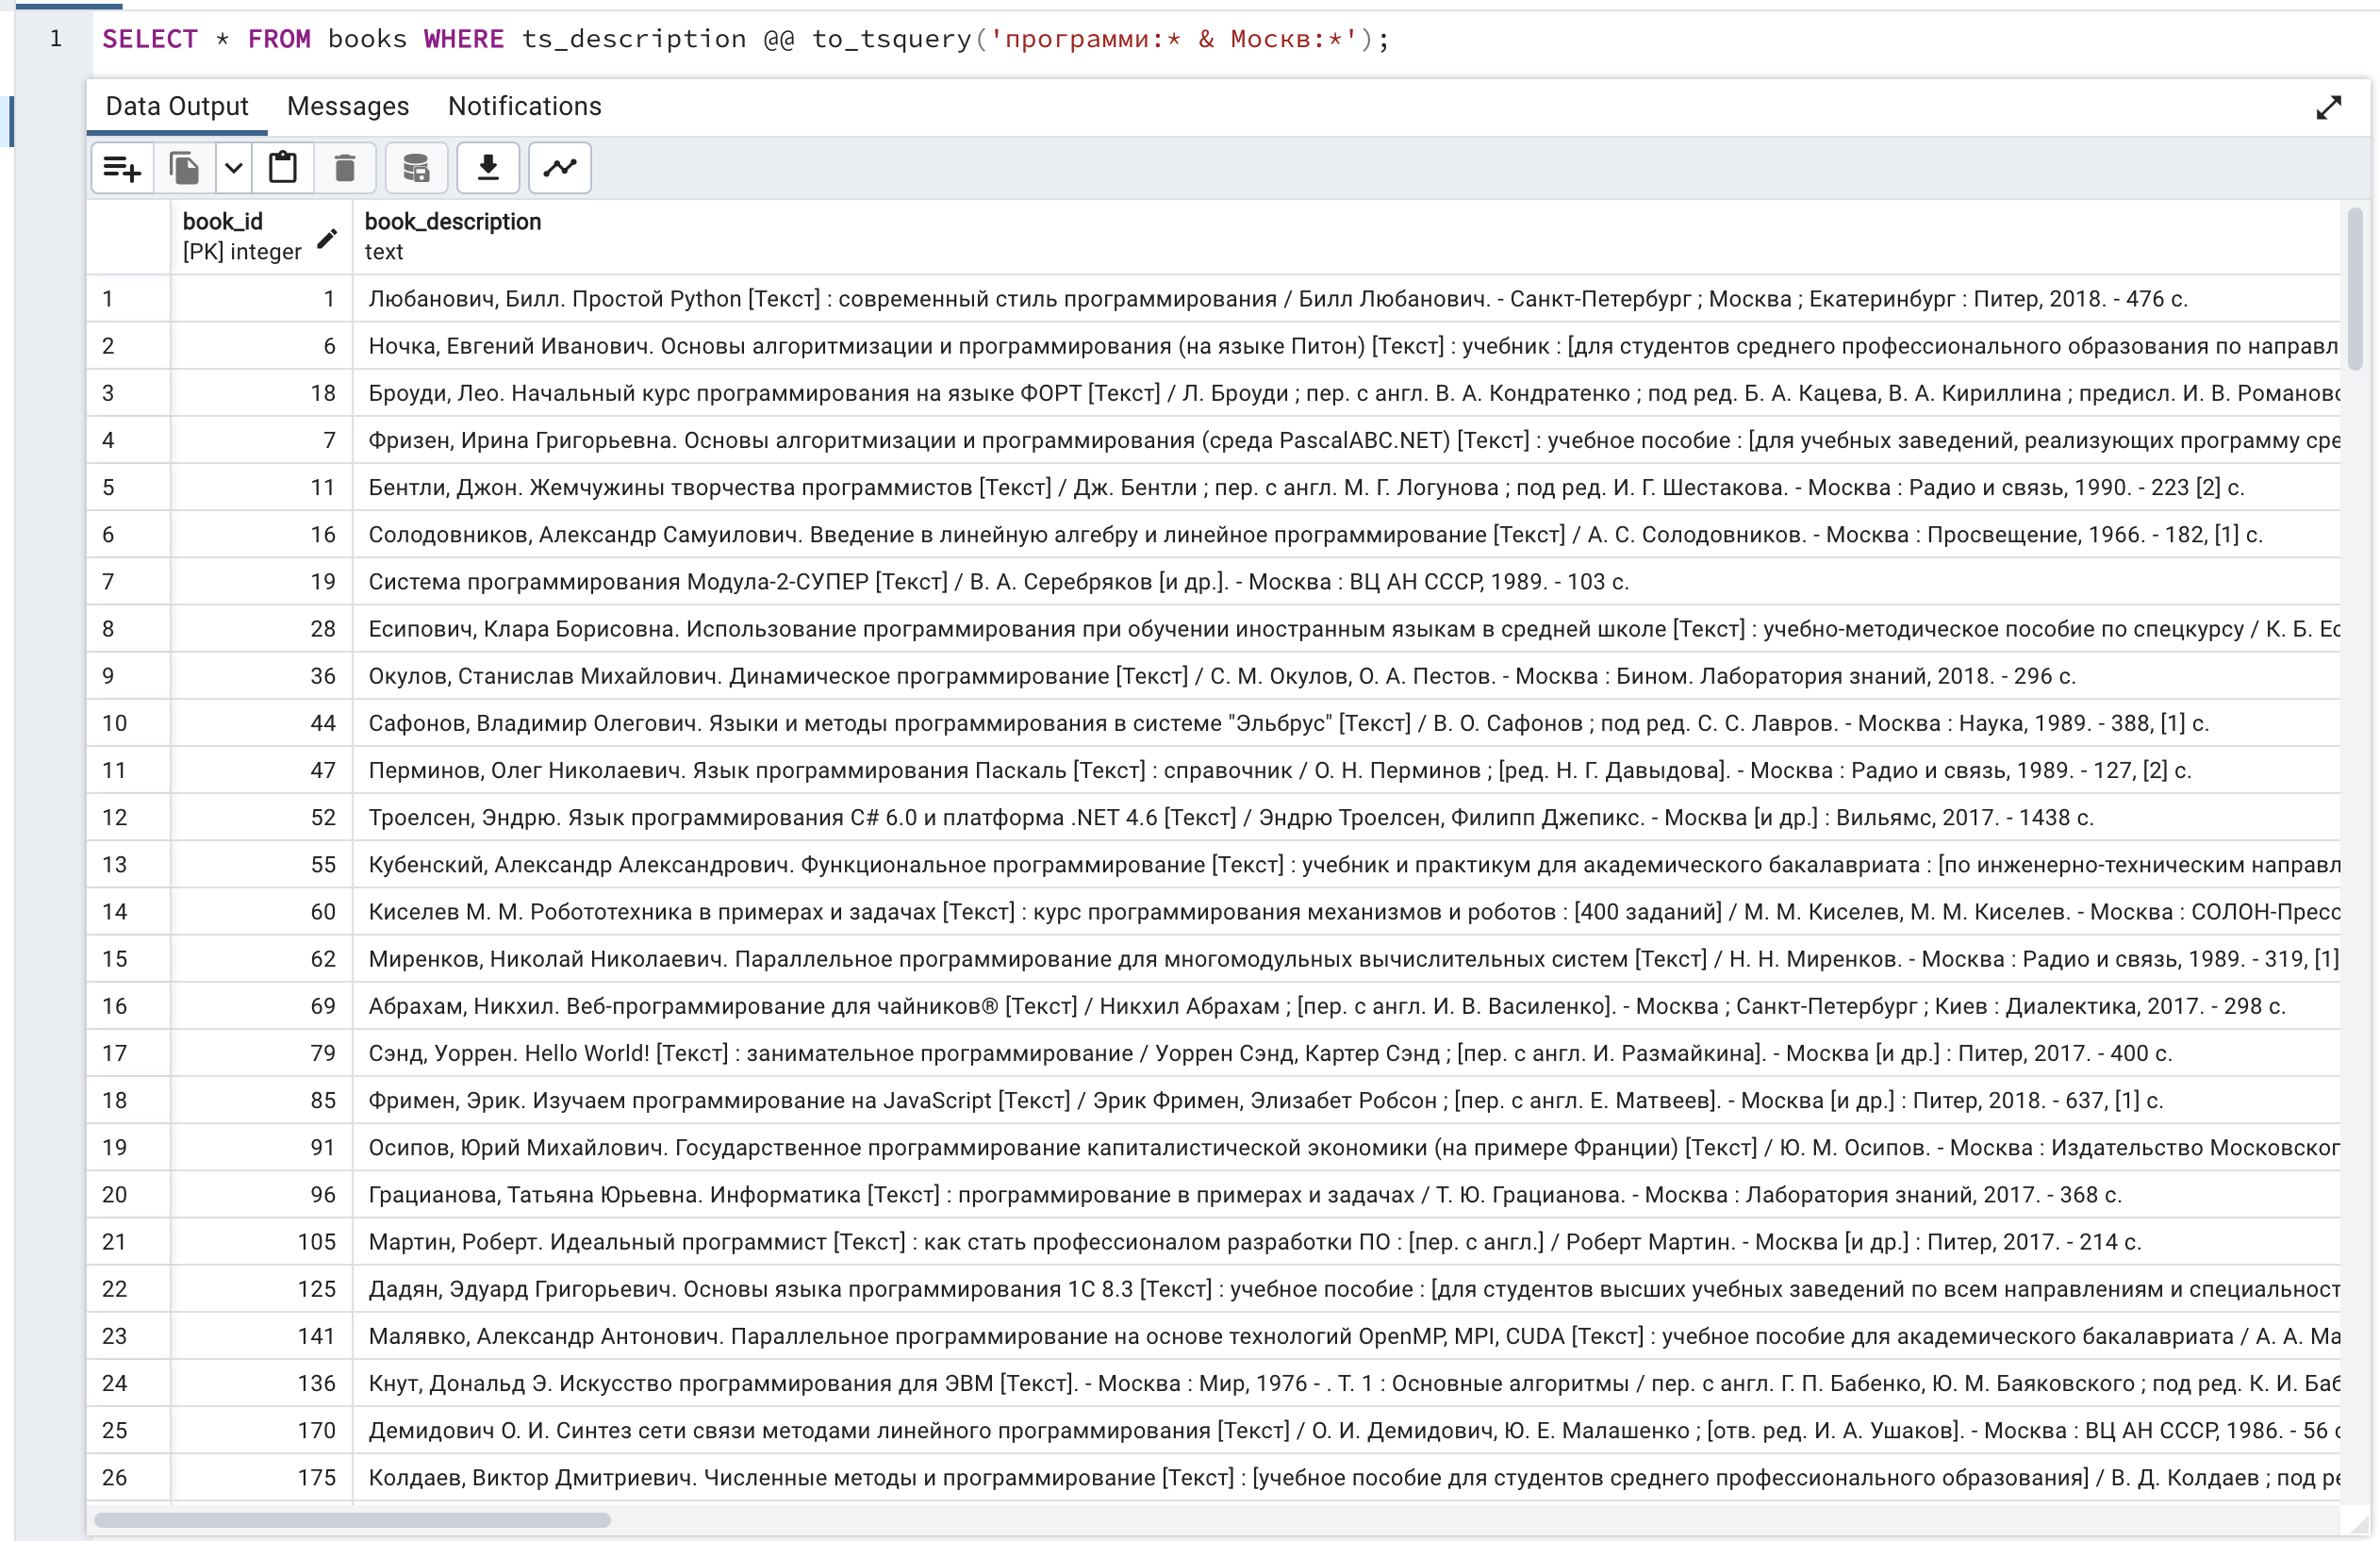
\includegraphics[scale=0.4]{3.png}
\end{center}
\clearpage
Книги про Python:
\begin{center}
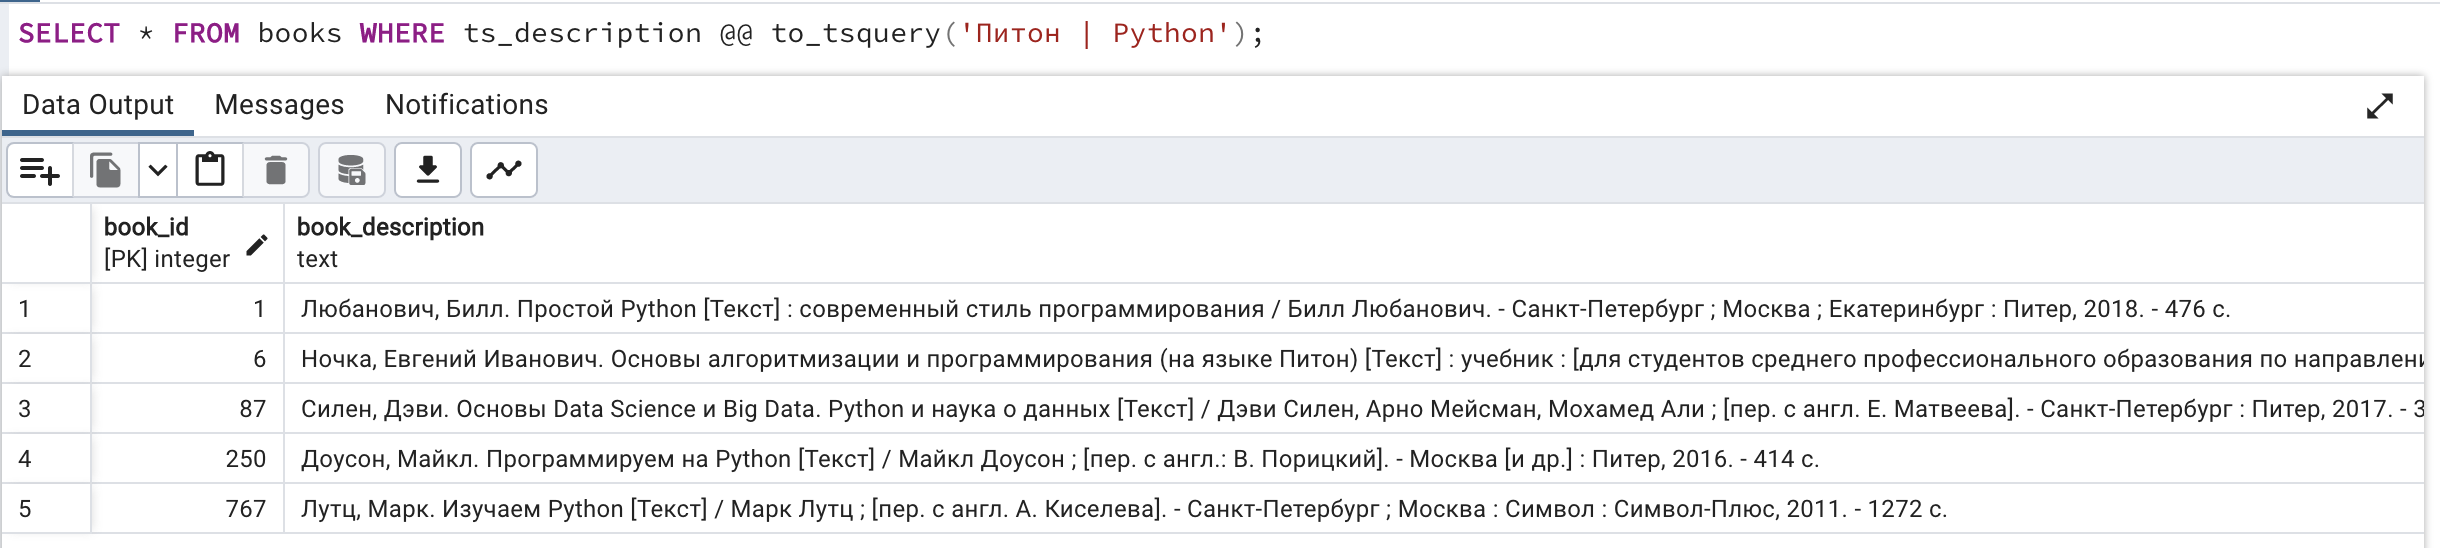
\includegraphics[scale=0.4]{4.png}
\end{center}
Книги для бакалавриата ИЛИ магистратуры:
\begin{center}
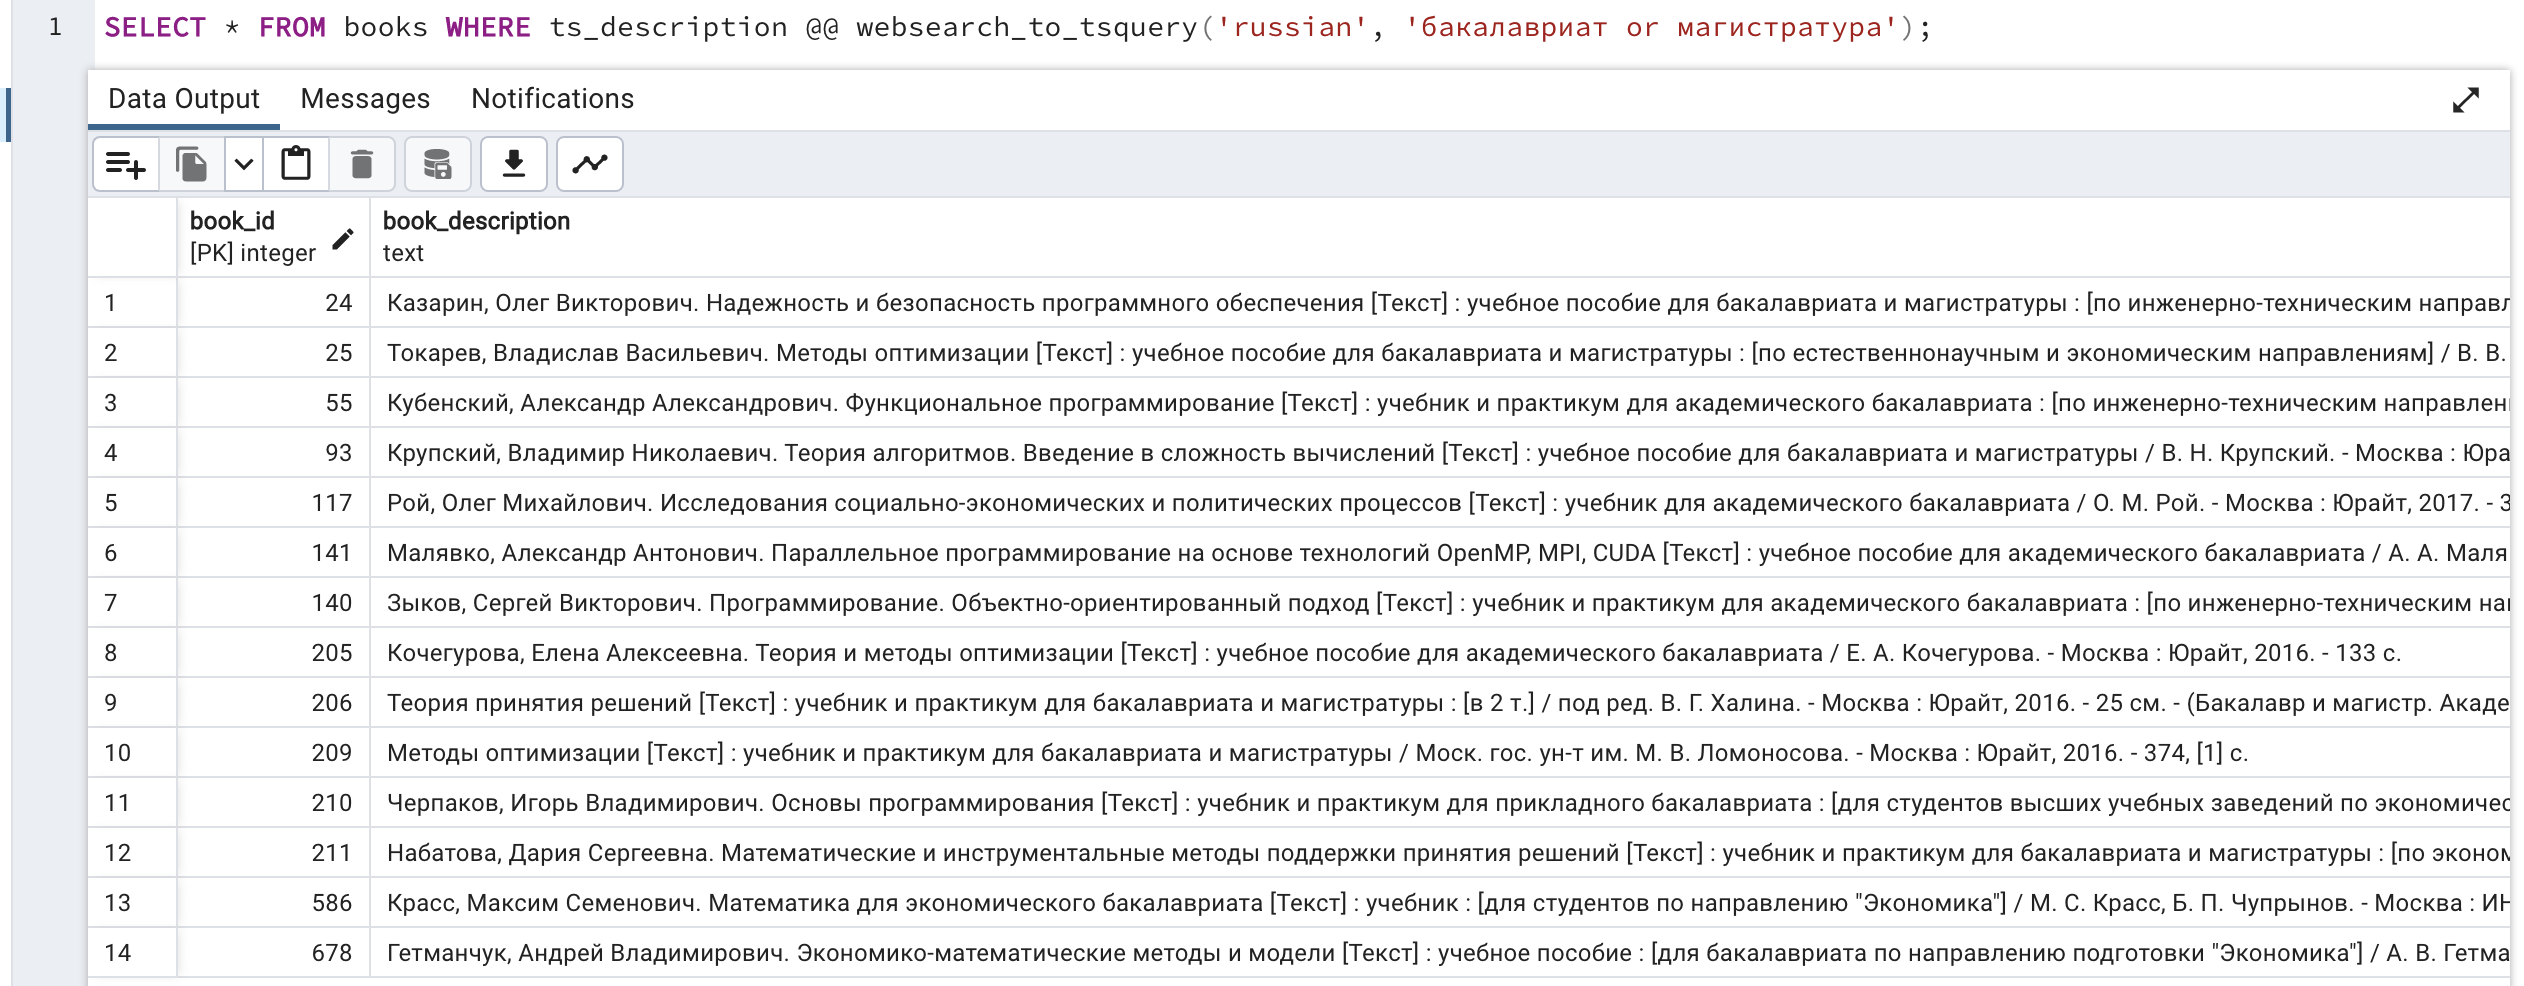
\includegraphics[scale=0.4]{5.png}
\end{center}
Книги от издательства Форум про язык Pascal (она всего одна):
\begin{center}
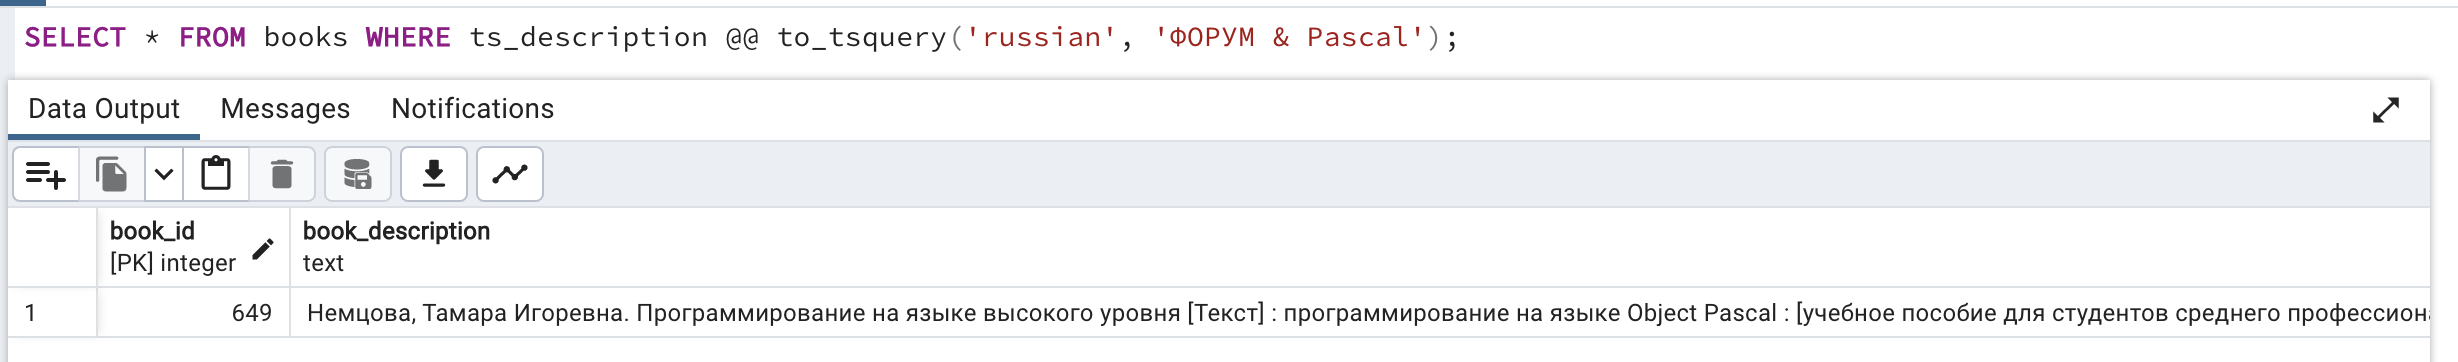
\includegraphics[scale=0.4]{6.png}
\end{center}
Книги, которые были написаны любым человеком с именем Григорий (такая тоже всего одна, к сожалению):
\begin{center}
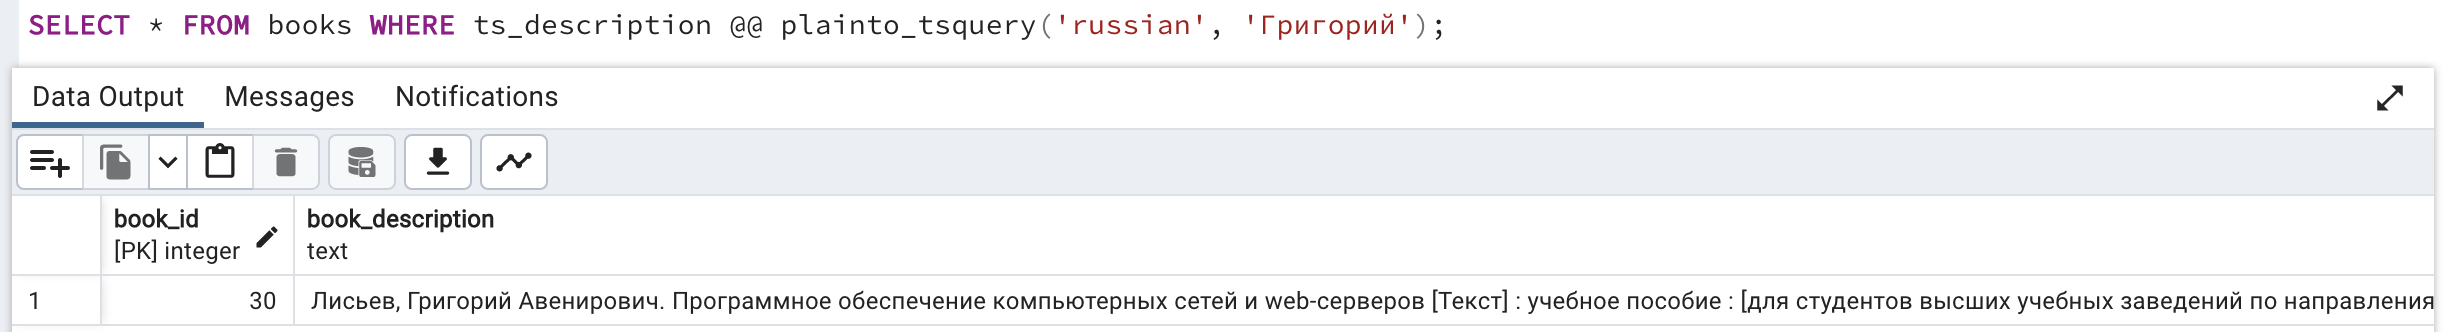
\includegraphics[scale=0.4]{7.png}
\end{center}
\end{document}
